\chapter{Impact: The Collision That Matters}
\label{ch:impact_collision_collision}

\section{The State Delivered to the Ball}

Impact converts part of the club's incident mechanical energy into ball
translation, spin, deformation, and dissipation. The golfer and club retain
energy afterward; the entire swing energy is not transferred in the collision.
Launch also depends on the local face normal, contact-point velocity, strike
location, ball and face properties, and the club's response during contact.
Ball speed, launch direction, launch elevation, and the full spin vector are
needed to initialize a flight model. Three scalars omitting speed and spin
axis cannot determine the trajectory.

For the rigid clubhead, let $O$ be its centre of mass and $P$ the contact point:
\begin{equation}
v_P=v_O+\omega_c\times r,\qquad r=p_P-p_O.
\end{equation}
Both velocities and all offsets must use the same frame. A path reported at
the face centre need not equal the centre-of-mass path. Face attitude is a
different quantity from velocity; static loft plus attack angle does not
determine dynamic loft. Declare whether delivery is measured immediately
before contact, at maximum compression, or at another instant.

\section{Normal Impact: Momentum, Restitution, and Energy}

For an isolated one-dimensional collision with stationary ball, club mass
$M$, ball mass $m$, and incident club speed $v$, momentum and restitution give
\begin{align}
Mv&=Mv_c^++mv_b^+,\label{eq:momentum_conservation}\\
e&=\frac{v_b^+-v_c^+}{v}.\label{eq:cor_definition}
\end{align}
This is relative separation speed divided by relative approach speed. A
coefficient from a fixed-surface rebound experiment requires its own setup
definition before being compared with a moving-club result.
Solving gives
\begin{equation}
v_b^+=\frac{(1+e)M}{M+m}v,\qquad
v_c^+=\frac{M-em}{M+m}v.
\label{eq:ball_velocity_after}
\end{equation}
For $M=0.200$ kg, $m=0.04593$ kg, and illustrative $e=0.83$, the speed
ratio is about $1.488$. This explains the scale of driver smash factor within
the model. It is not a universal equipment ceiling or a direct energy ratio.

The ball's fraction of initial club translational energy is
\begin{equation}
\frac{E_b^+}{E_c^-}=\frac{m}{M}
\left[\frac{(1+e)M}{M+m}\right]^2,
\end{equation}
about $0.508$ for those values. The total kinetic-energy loss is
\begin{equation}
E^- - E^+=\tfrac12\frac{Mm}{M+m}(1-e^2)v^2.
\end{equation}
Thus $e^2$ describes retained relative-motion energy in the centre-of-mass
frame for this model; it is not the fraction of club energy delivered to the
ball. Oblique impact also partitions energy into rotation and deformation.
These distinctions underlie standard golf impact treatments~\citep{Jorgensen1994,Penner2003}.

\begin{figure}[htbp]
\centering
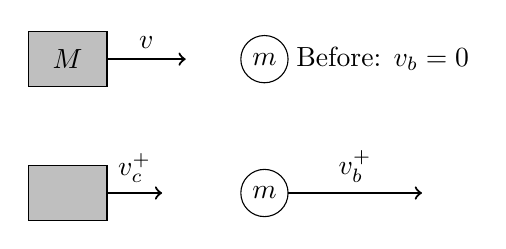
\begin{tikzpicture}
\draw[fill=lightgray] (0,1) rectangle (1,1.7);
\node at (0.5,1.35) {$M$};
\draw[->,thick] (1,1.35) -- (2,1.35) node[midway,above] {$v$};
\draw (3,1.35) circle (0.3); \node at (3,1.35) {$m$};
\node at (4.5,1.35) {Before: $v_b=0$};
\draw[fill=lightgray] (0,-0.7) rectangle (1,0);
\draw[->,thick] (1,-0.35) -- (1.7,-0.35) node[midway,above] {$v_c^+$};
\draw (3,-0.35) circle (0.3); \node at (3,-0.35) {$m$};
\draw[->,thick] (3.3,-0.35) -- (5,-0.35) node[midway,above] {$v_b^+$};
\end{tikzpicture}
\caption{Isolated One-Dimensional Impact Before and After Contact. Momentum and Relative-Speed Restitution Determine Both Outgoing Velocities.}
\label{fig:impact_collision}
\end{figure}

\section{Effective Mass and Off-Centre Impact}
\label{sec:ch28_effective_mass}

For a free rigid clubhead, an impulse $J\hat n$ produces translational and
rotational changes. With inertia tensor $I_c$ about its centre of mass,
\begin{equation}
\frac{1}{M_{\rm eff}}=\frac1M+
(r\times\hat n)^T I_c^{-1}(r\times\hat n).
\end{equation}
The second term is nonnegative, so $M_{\rm eff}\le M$. It vanishes when
the impulse line passes through the centre of mass, even if the contact point
is some distance in front of it. Effective mass is directional inertial
response, not the amount of material physically reached by a wavefront.

For a multibody model with mass matrix $M_q$ and contact Jacobian $J_P$,
the corresponding directional inverse mass is
$\hat n^TJ_PM_q^{-1}J_P^T\hat n$, modified by active constraints.
Flexible modes, boundary conditions, and contact duration require a compatible
dynamic model. There is no general rule that shaft and arm coupling always
add 10--20 percent to clubhead effective mass.

Off-centre impact changes head rotation, contact velocity, and tangential
impulse. This produces gear effect. Local face bulge and roll also change the
normal, while face compliance can vary with strike position. Ball-speed loss
cannot universally be assigned to only one of these mechanisms.

\section{Oblique Contact and Spin}

Let $\hat n$ point from face into ball and split impulse into normal and
tangential components. Neglecting other impulses over the short contact,
\begin{align}
m\Delta v_b&=J_n\hat n+J_t,\\
I_b\Delta\omega_b&=r_b\times(J_n\hat n+J_t).
\end{align}
For an ideal sphere of radius $R$, $r_b=-R\hat n$. A centred normal impulse
then produces no spin, while the tangential impulse produces angular momentum.
A finite contact patch can also transmit a torsional moment that the point
contact model omits.

Coulomb friction supplies a bound $\|F_t\|\le\mu F_n$, with equality in
ideal gross sliding. Sticking does not imply zero friction. Tangential
deformation, partial slip, and restitution can continue after gross slip
ceases, so a rigid rolling condition does not universally fix outgoing spin.
Contact properties must be identified at relevant speed, loading, and surface
conditions. A low-speed ball-on-granite experiment is not a direct driver
calibration.

More obliqueness does not guarantee monotonically increasing spin. Sliding,
normal impulse, tangential compliance, moisture, and strike location can change
the trend. Grooves help manage contamination, but a universal spin increment
from groove count or loft alone is not supplied by this model.

\section{Exact Spin-Loft Geometry}

Use a forward/up/right frame, face azimuth $\phi$, path azimuth $\psi$,
dynamic loft $\lambda$, and attack angle $\alpha$. The unit vectors are
\begin{align}
\hat n&=(\cos\lambda\cos\phi,\sin\lambda,\cos\lambda\sin\phi),\\
\hat v&=(\cos\alpha\cos\psi,\sin\alpha,\cos\alpha\sin\psi).
\end{align}
Spin loft is their angle:
\begin{equation}
\cos\Phi=\sin\lambda\sin\alpha+
\cos\lambda\cos\alpha\cos(\phi-\psi).
\end{equation}
For zero face-to-path, $\Phi=|\lambda-\alpha|$ in the relevant range.
Otherwise, multiplying $\cos(\phi-\psi)$ by $\cos(\lambda-\alpha)$ is not
the exact identity. Nor can a horizontal path angle be subtracted from loft
to obtain spin loft.

With measured dynamic loft $12^\circ$, attack $2.5^\circ$, and square
face-to-path, spin loft is $9.5^\circ$. If an illustrative vertical launch
weighting is $0.84$ toward the normal and $0.16$ toward the velocity,
launch elevation is $0.84(12)+0.16(2.5)=10.48^\circ$.
The weighting is empirical, not a universal law. Spin rate and carry require
additional contact and flight inputs. With face azimuth fixed, changing path
from $-3^\circ$ to $+3^\circ$ preserves spin loft by symmetry but reverses
the ideal horizontal spin tendency; it does not subtract three degrees of loft.

For a centred symmetric impact on a nonspinning ball, the ideal spin direction
is parallel to $\hat v\times\hat n$. The cross product degenerates at zero
obliquity. Use its projections in a declared launch frame to calculate axis
tilt; a tan/tan rule is not a general three-dimensional identity. Gear effect
and asymmetric or rotating contact require additional terms.

In a normal-only model with $C=(1+e)/(1+m/M_{\rm eff})$,
$v_b=C(v_P\cdot\hat n)\hat n$. Total ball speed scales with $\cos\Phi$;
its projection onto incident velocity scales with $\cos^2\Phi$. Those are
different outputs. A tangential impulse modifies both direction and speed.

\section{How Isolated Is the Collision?}

The relevant comparison is impulse. An external force $F(t)$ contributes
$\int F\,dt$, which must be compared with the ball-contact impulse in the
same direction and model boundary. For an illustrative $300$ N acting
unchanged over $0.5$ ms, the impulse is $0.15$ N s. A $0.04593$ kg ball
leaving at $67$ m/s gains approximately $3.08$ N s. This comparison is a
scale estimate, not a measured grip-to-ball sensitivity: grip forces may not
reach the head with that magnitude or direction.

Axial wave speed $c=\sqrt{E/\rho}$ in a uniform slender rod differs from
frequency-dependent bending-wave propagation. Wave arrival time establishes
neither force amplitude nor the resulting change in launch speed. Existing
shaft deformation, head inertia, grip impedance, reflection, and contact
dynamics must be modeled together. An assumed spring deflection multiplied
by stiffness cannot by itself prove a percentage change in effective mass.

The short collision leaves no time for a new consciously selected response to
that collision to influence it. Existing activation, preprogrammed commands,
intrinsic tissue forces, and mechanical boundary conditions nevertheless remain.
This distinction is especially important in the preceding tens of milliseconds:
brief ball contact does not establish an unactuated final 50--100 ms of downswing.

\section{A Precise Counterfactual Question}
\label{sec:ztcf_impact}

A smooth pre-impact model may be written $\dot x=f(x)+G(x)u$ for declared
state, inputs, and constraints. The collision can be represented by a reset
$x^+=\Delta(x^-)$ or by resolved compliant contact. It is not automatically
the same smooth drift field continued through an impulsive event.

To isolate earlier actuation, branch before impact, specify which torques or
excitations are removed, and evolve each branch with its own contact event.
To isolate grip boundary mechanics during impact, hold the pre-impact state
fixed and vary only the declared boundary model. These are different
experiments. A peak collision-force/grip-force ratio is not a bound on
reachable states, a work fraction, or evidence that muscle control has ceased.

\section{Measurement and Model Checks}

\begin{enumerate}
\item Declare the contact point, normal, reference point for club velocity,
and measurement instant. Include their uncertainty and time synchronization.
\item Compare impulse integrals with linear and angular momentum changes.
Do not infer moment solely from a force magnitude without its line of action.
\item Check both bodies' post-impact energy. A fitted restitution coefficient
must not create unexplained energy in an otherwise passive model.
\item Validate ball speed, launch angles, spin magnitude and axis together.
Fitting one outcome does not validate the others.
\item Vary integration step and contact resolution for compliant models;
report convergence of impulses, energy residual, and launch conditions.
\item Separate equipment conformance tests from ball-contact experiments.
Characteristic time from a steel pendulum is not golf-ball contact duration.
\end{enumerate}

\section{Connecting Swing Mechanics to Ball Flight}

Earlier joint work and energy transfer help create incident club motion.
Geometry and wrist control help determine local contact velocity and face
attitude. Shaft deformation contributes to the delivered state and boundary
response. The collision maps those inputs into launch; aerodynamics, wind,
and the landing surface determine later flight and roll. This chain explains
why a swing theory should predict a distribution of impact states and measured
launch outcomes, rather than declaring one isolated motion variable optimal.

\section{Exercises}
\begin{enumerate}
\item Use $M=0.200$ kg, $m=0.04593$ kg, $v=50$ m/s, $e=0.83$ to compute
both outgoing velocities, the ball's energy fraction, and total energy loss.
Verify momentum conservation independently.
\item At fixed inertia, compare directional effective mass for an impulse
through the centre of mass and one with a perpendicular offset. Explain why
distance from the face to the centre of mass alone is insufficient.
\item Compute exact spin loft for $\lambda=40^\circ$, $\alpha=20^\circ$,
and face-to-path $30^\circ$, then quantify the error in the product-of-cosines shortcut.
\item Distinguish total ball speed from its forward projection at $30^\circ$
obliquity in the normal-only model.
\item Design a matched-state grip-boundary experiment. Specify which measured
changes would falsify the claim that grip mechanics are negligible at the chosen accuracy.
\end{enumerate}
